\documentclass[a4paper]{scrartcl}
%\usepackage{tikz}
\usepackage[
typ={kl},
fach=Informatik,
farbig
]{schule}
\hypersetup{hidelinks}


%\usepackage{ctable}
%
%´\usepackage[default]{fontsetup}

\usepackage[default]{fontsetup}
%\usepackage{fontspec}
%\usepackage{fourier-otf}
%\setmonofont{FiraCode-Regular}[
%Contextuals=Alternate % Activate the calt feature
%]
%\usepackage{newunicodechar}
%\newunicodechar{^^^^2588}{█}
%\newunicodechar{█}{█}
%\setmonofont{Fira Code}
%\usepackage{amsmath}
%\usepackage{amssymb}
%\setmonofont{Ubuntu Mono Regular}[Scale=0.9]
%\usepackage{pmboxdraw}
%\usepackage{cascadia-code}
%\usepackage[scale = 0.1]{jetbrainsmono-otf}
%\usepackage{cascadiamono-otf}
%\setmonofont{CascadiaMono-SemiLight}[]
\usepackage{monaspace-otf}
%\setmonofont[Scale = MatchLowercase]{jetbrainsmono-light}
%\newunicodechar{2588}{█}
%\newunicodechar{█}{\pmboxdrawuni{2588}}

\usepackage{scrlayer-scrpage}
\ifoot{% TODO: \usepackage{graphicx} required
	
	
\includegraphics[width=0.15\linewidth]{GHSE-Logo}
	
}

\usepackage[ngerman]{babel} 

\usepackage{shellesc}
\usepackage{minted}

\usepackage{microtype}	

\usepackage{fancyvrb}
\date{}

\title{IFT KA4 TGI12}
\begin{document}

\punktuebersicht


Sie möchten ihre Studentenbude smart machen und beginnen damit, ihr
Wohnzimmer mit smarten Geräten auszustatten.

Sie verfügen bereits über zwei intelligente Heizungsregler. Mit diesen lässt sich die
Raumtemperatur regeln.

Außerdem haben sie drei Lampen in ihrem Wohnzimmer smart gemacht. Diese
lassen sich in der Helligkeit zwischen $0-100 \%$ regeln. Darüber hinaus kann die Lichtfarbe der RGB-Lampen
gewählt werden.

Die Rollos des Fensters und der
Balkontür lassen sich ebenfalls
über ihre Smart Home Zentrale
steuern. Die Rollos können
zwischen $0-100\%$ geöffnet bzw.
geschlossen werden.

Ihr WLAN, TV und MP3-Player
lassen sich ebenfalls über die
App steuern. Auf der Oberfläche
ihrer App können sie die
einzelnen Geräte auswählen.
% TODO: \usepackage{graphicx} required
\begin{figure}[H]
\centering
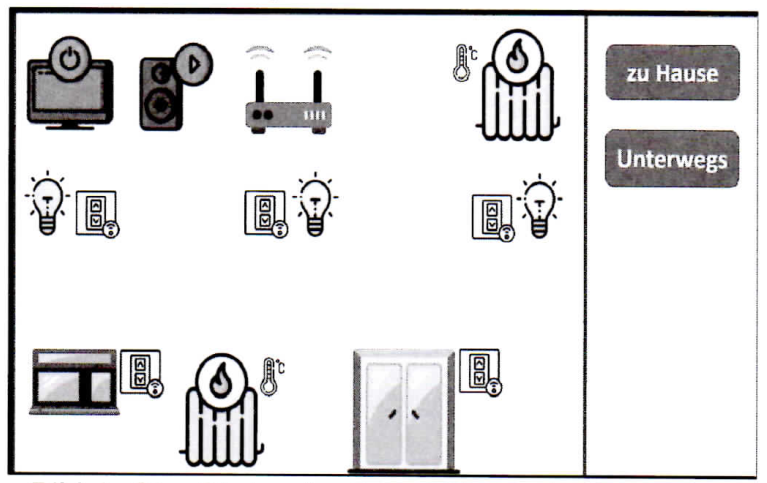
\includegraphics[width=0.7\linewidth]{bild}
\caption{}
\label{fig:bild}
\end{figure}




Ein unvollständiges Klassendiagramm liegt bereits vor, siehe Abbildung 3. Tragen
Sie die Lösungen der zwei folgenden Aufgabenteile darauf ein.

Sie kommen von der Vorlesung nach Hause und wollen, dass es in ihrem Wohnzimmer
gemütlich ist (Temperatur, Licht, ...).

Dafür haben sie sich auf der Oberfläche der App einen Button »zu Hause" angelegt
(Abbildung 1). Durch Betätigen dieses Buttons werden die gewünschten Einstellungen an die
Geräte übermittelt. Geräte, die über die Eigenschaft \texttt{status} verfügen, können
eingeschaltet werden, indem \texttt{status} auf \texttt{true} gesetzt wird.

Der Vorgang ist im Sequenzdiagramm in Abbildung 2 dargestellt.

% TODO: \usepackage{graphicx} required
\begin{figure}
\centering

\includegraphics[width=1.3\linewidth, angle=90]{sequenzdiagramm_1}
\caption{}
\label{}
\end{figure}

% TODO: \usepackage{graphicx} required
\begin{figure}
\centering

\includegraphics[width=\linewidth]{kd}
\caption{}
\label{fig:kd}
\end{figure}

\begin{aufgabe}[points=9]
Ergänzen Sie das Klassendiagramm mit allen Assoziationen, die sich aus dem
Sequenzdiagramm ergeben. Tragen Sie für jede Assoziation die Richtung, den
Rollennamen sowie die Multiplizität ein.

\hinweis{Bei manchen Multiplizität musst du genau lesen/hinschauen!}
\end{aufgabe}

\begin{aufgabe}[points=7]
Überprüfen Sie, ob alle Botschaften des Sequenzdiagramms aus Abbildung 2 als
Operationen im Klassendiagramm berücksichtigt sind.

Ergänzen Sie fehlende Operationen mit vollständiger Signatur, dem Rückgabewert und
der Sichtbarkeitskennzeichnung.
\end{aufgabe}


\begin{aufgabe}[points=1]
Die an das System angeschlossenen Geräte (Heizungen, Rollladen und Lampen)
verfügen über keinen LAN-Anschluss, d.h. die Datenübertragung erfolgt per WLAN.
Das in dem Sequenzdiagramm aus Abbildung 2 beschriebene Verhalten kann in der Realität
nicht funktionieren.

Finden Sie den logischen Fehler und beschreiben Sie einen Lösungsvorschlag.
\end{aufgabe}


\begin{aufgabe}[points=2]
Erkläre was der Zusatz zum Attribut \texttt{weg} der Klasse \texttt{Rolladen} bedeutet.
\end{aufgabe}

\begin{aufgabe}[points=15]
Wenn Sie das Haus verlassen, benutzen Sie den Button \texttt{Unterwegs} (Abbildung 1), um die
Wohnung abzusichern. Dem System wurden weitere Melder hinzugefügt, die in den
Klassendiagrammen in letzten Aufgaben nicht dargestellt sind. Diese haben aber
den gleichen Aufbau wie die anderen Melder. Die Steuerung hat zu
jedem Melder eine Assoziation.

Entwerfen Sie ein Sequenzdiagramm in UML-Notation mit konkreten Parameterwerten
für folgendes Szenario. Nutzen sie dabei die Vorlage.


\begin{itemize}
\item In ihrer Wohnung gibt es drei Bewegungsmelder (Klasse \texttt{BMelder}). Diese sollen
mit Hilfe der Methode \texttt{setStatus(true)} aktiviert werden.
\item  In Ihrer Wohnung gibt es darüber hinaus an der Eingangstür, der Terrassentür
und den drei Fenstern jeweils einen Tür- bzw. Fenstersensor (Klasse
\texttt{TFMelder}). Diese sollen mit Hilfe der Methode \texttt{setStatus(true)} ebenfalls aktiviert werden.
\item  Die Temperatur der beiden Heizungen wird mit 21° ermittelt und dann auf 19°
eingestellt.
\item Alle drei Lampen werden ausgeschaltet.
\item Das WLAN wird ausgeschaltet.
\end{itemize}
\end{aufgabe}


% TODO: \usepackage{graphicx} required
\begin{figure}[H]
\raggedright

\includegraphics[width=0.23\linewidth]{sequenzdiagramm_vorlage}
\label{fig:sequenzdiagramm_vorlage}
\end{figure}

\pagebreak

\begin{minted}{java}
import java.util.EmptyStackException;

record Node<T> (T content, Node<T> nextNode) {}

public class SimpleStack<T> {
    private Node<T> first;

    public SimpleStack() {
        this.first = null;
    }

    public void push(T x) {
        first = new Node<T>(x, first);
    }

    public T pop() {
        if (first == null) throw new EmptyStackException();
        var result = first.content();
        first = first.nextNode();
        return result;
    }
}

record ToDo(String text, boolean done) {
    ToDo(String text){
        this(text, false);
    }
}


void main(){
   var s = new SimpleStack<ToDo>();
   s.push(new ToDo("IFT-Hausaufgaben"));
   s.push(new ToDo("App programmieren"));
   s.pop();
   s.push(new ToDo("Weltherrschaft übernehmen"));
   // Objektdiagramm
   // ..
}
\end{minted}


\begin{aufgabe}[points=9]
Stelle den Zustand in der Zeile mit dem Kommentar \texttt{// Objektdiagramm} als Objektdiagramm dar.
\end{aufgabe}

\end{document}
